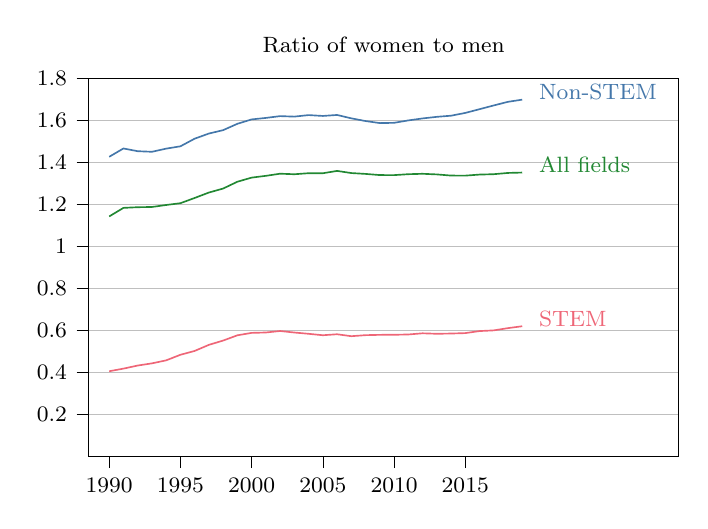
\begin{tikzpicture}[every node/.style={font=\footnotesize},
align=left]
% This file was created with tikzplotlib v0.9.17.
\definecolor{color0}{rgb}{0.266666666666667,0.466666666666667,0.666666666666667}
\definecolor{color1}{rgb}{0.933333333333333,0.4,0.466666666666667}
\definecolor{color2}{rgb}{0.133333333333333,0.533333333333333,0.2}

\begin{axis}[
height=6.376357092455836cm,
tick align=outside,
tick pos=left,
title={Ratio of women to men},
width=9.079103cm,
x grid style={white!69.0196078431373!black},
xmin=1988.55, xmax=2030,
xtick style={color=black},
xtick={1990,1995,2000,2005,2010,2015},
xticklabels={
  \(\displaystyle 1990\),
  \(\displaystyle 1995\),
  \(\displaystyle 2000\),
  \(\displaystyle 2005\),
  \(\displaystyle 2010\),
  \(\displaystyle 2015\)
},
ymajorgrids,
ymin=0, ymax=1.8,
ytick style={color=black},
ytick={0.2,0.4,0.6,0.8,1,1.2,1.4,1.6,1.8},
yticklabels={
  \(\displaystyle 0.2\),
  \(\displaystyle 0.4\),
  \(\displaystyle 0.6\),
  \(\displaystyle 0.8\),
  \(\displaystyle 1\),
  \(\displaystyle 1.2\),
  \(\displaystyle 1.4\),
  \(\displaystyle 1.6\),
  \(\displaystyle 1.8\)
}
]
\addplot [semithick, color0]
table {%
1990 1.427405505634
1991 1.46714809099813
1992 1.45408856644051
1993 1.45133056069635
1994 1.46632675500279
1995 1.47745338056048
1996 1.51376718247216
1997 1.53828798725427
1998 1.55449336861595
1999 1.58473297320645
2000 1.60565375757982
2001 1.61278508325131
2002 1.62135031330213
2003 1.61899720890419
2004 1.62626691016731
2005 1.62216110347127
2006 1.6268814689671
2007 1.61078767056739
2008 1.59785935029602
2009 1.58812505042948
2010 1.58941530974578
2011 1.60087854553429
2012 1.61034082337528
2013 1.61796341316566
2014 1.62335431427331
2015 1.63658821029616
2016 1.65433859998146
2017 1.67230386982575
2018 1.68955365020253
2019 1.69994419498014
};
\addplot [semithick, color1]
table {%
1990 0.405000888257239
1991 0.417524255351278
1992 0.43220401589811
1993 0.442613861386139
1994 0.456943044266005
1995 0.483474314581324
1996 0.50180214068324
1997 0.530851247368966
1998 0.551297608869522
1999 0.576324444351342
2000 0.587942253646939
2001 0.589702386485876
2002 0.596825233144927
2003 0.589620930726998
2004 0.583512711965751
2005 0.576685418077931
2006 0.581362635810389
2007 0.572103909345816
2008 0.577021785915687
2009 0.578571146701844
2010 0.578888552981062
2011 0.580283660424367
2012 0.585892143871724
2013 0.583614442637939
2014 0.584783566354309
2015 0.586807592049527
2016 0.596514797507788
2017 0.599850220979392
2018 0.610571281705869
2019 0.619632027676551
};
\addplot [semithick, color2]
table {%
1990 1.14299510342925
1991 1.18391649994092
1992 1.18704801250989
1993 1.18813211258767
1994 1.19766422919376
1995 1.20619843240183
1996 1.23111660416933
1997 1.25700638354037
1998 1.27605686630601
1999 1.30854746295602
2000 1.32815535799601
2001 1.33665603902656
2002 1.34681270324835
2003 1.34425840993905
2004 1.34918302107431
2005 1.34898299997691
2006 1.36012601962975
2007 1.34989624835205
2008 1.34579743339092
2009 1.34033067525664
2010 1.34007741777359
2011 1.34444943301349
2012 1.3464106865242
2013 1.34343483847832
2014 1.33796617858431
2015 1.33759763166717
2016 1.34265313826302
2017 1.34451026998746
2018 1.35044521494211
2019 1.35227525265305
};
\draw (axis cs:2019.5,1.69994419498014) node[
  anchor=base west,
  text=color0,
  rotate=0.0
]{Non-STEM};
\draw (axis cs:2019.5,0.619632027676551) node[
  anchor=base west,
  text=color1,
  rotate=0.0
]{STEM};
\draw (axis cs:2019.5,1.35227525265305) node[
  anchor=base west,
  text=color2,
  rotate=0.0
]{All fields};
\end{axis}



\end{tikzpicture}

\caption{STEM fields include: agriculture and related sciences; natural resources and conservation; computer services; engineering; engineering technologies; biological sciences; mathematics and statistics; physical sciences;  and science technologies. Source: IPEDS.}
